%  !TeX  root  =  user_guide.tex

\chapter{Lavorare con le proiezioni}\label{label_projections}
\index{Projections!working with}

% when the revision of a section has been finalized,
% comment out the following line:
%\updatedisclaimer

QGIS consente all'utente di definire un CRS (Coordinate Reference System, ovvero Sistema di Coordinate di Riferimento) 
globale o a livello di singolo progetto, per i layer privi di un CRS predefinito. Consente inoltre di definire sistemi 
di coordinate personalizzati e supporta la riproiezione al volo (on-the-fly, OTF) dei layer vettoriali. Tutte queste 
caratteristiche permettono all'utente di visualizzare contemporaneamente layer aventi CRS differenti, correttamente 
sovrapposti.

\section{Panoramica del supporto alle proiezioni}\label{label_projoverview}

QGIS supporta all'incirca 2.700 CRS noti. Le definizioni di ognuno di questi CRS sono immagazzinate in un database SQLite 
che viene installato con QGIS. Normalmente non è necessario manipolare il database direttamente, infatti questa operazione 
può causare il malfunzionamento del supporto alla proiezione. I CRS personalizzati sono salvati in un database utente.
Si veda la sezione \ref{sec:customprojections} per informazioni sulla gestione dei CRS personalizzati.

I CRS disponibili in QGIS sono basati su quelli definiti da EPSG\index{EPSG} e sono per lo più tratti dalle tabelle 
spatial\_references di PostGIS\index{PostGIS} versione 1.x. Gli identificatori EPSG sono presenti nel database e 
possono essere usati per richiamare e definire i CRS in QGIS.

Per usare la riproiezione al volo (OTF), i dati devono contenere informazioni sul proprio sistema di
coordinate oppure bisogna definire un CRS per il layer, a livello di progetto oppure globale. Per i layer 
PostGIS, QGIS usa l'identificatore del riferimento spaziale specificato al momento della creazione del layer.
Per i dati supportati da OGR, QGIS fa affidamento sulla presenza di un mezzo, specifico per ciascun formato, 
che definisce il CRS. Nel caso degli shapefile, questo significa un file che contiene l'indicazione del CRS 
in formato Well Known Text (WKT)\index{WKT}. Il file della proiezione ha lo stesso nome dello shapefile, ma 
ha estensione prj. Per esempio uno shapefile chiamato \filename{alaska.shp} avrà un corrispondente file 
di proiezione chiamato \filename{alaska.prj}.

Ogni volta che si seleziona un nuovo CRS, le unità utilizzate per il layer verranno automaticamente aggiornate 
nella scheda \tab{Generale} della finestra di dialogo \dropmenuopttwo{mActionOptions}{Proprietà Progetto} 
sotto il menu \mainmenuopt{Modifica} (Gnome, OS X) o \mainmenuopt{Impostazioni} (KDE, Windows).

\section{Specificare una proiezione}
\index{Projections!specifying}
\label{sec:projection-specifying}

QGIS non imposta più il CRS della mappa al sistema di coordinate del primo 
layer caricato. Quando si avvia una sessione QGIS con layer privi di CRS, 
è necessario innanzitutto controllare e definire il CRS di questi layer. 
Questo può essere fatto globalmente o a livello di progetto nella scheda \tab{CRS} 
sotto la voce di menu \mainmenuopt{Impostazioni} \arrow \dropmenuopttwo{mActionOptions}{Opzioni} (KDE, Windows).
Si veda la Figura ~\ref{fig:crsdialog}.

\begin{itemize}[label=--]
\item \checkbox{Richiedi CRS}
\item \checkbox{CRS predefinito utilizzato dal progetto}
\item \checkbox{Verrà utilizzato il CRS globale predefinito visualizzato qui sotto}
\end{itemize}

In QGIS, il CRS globale predefinito è \texttt{proj=longlat +ellps=WGS84 +datum=WGS84+no\_defs}
ma può essere cambiato, e la nuova impostazione verrà salvata per le successive sessioni.

\begin{figure}[ht]
   \centering
   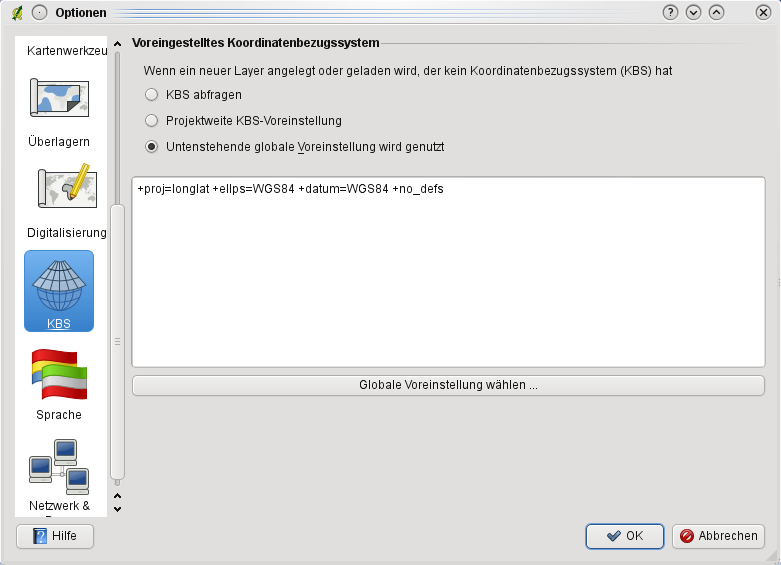
\includegraphics[clip=true, width=12cm]{crsdialog}
   \caption{Scheda CRS nella finestra opzioni di QGIS \nixcaption}\label{fig:crsdialog}
\end{figure}

Per definire il CRS di un layer privo di tale informazione, si può anche agire nella scheda \tab{Generale}
della finestra delle proprietà raster (\ref{label_generaltab}) e delle proprietà vettore (\ref{vectorgeneraltab}). 
Se il CRS è già stato definito, verrà mostrato come nella figura ~\ref{fig:vector_symbology}.

\section{Definire la riproiezione al volo (OTF)}\label{label_projstart}

In QGIS la riproiezione al volo (OTF) non è abilitata di default, e questa funzione è attualmente
supportata solo per i layer vettoriali. Per usare la riproiezione OTF, bisogna aprire la finestra
di dialogo \dropmenuopttwo{mActionOptions}{Proprietà Progetto}, selezionare un CRS e attivare la casella di controllo
\checkbox{Abilita la riproiezione al volo}.
Ci sono due modi per aprire questa finestra:

\begin{enumerate}
\item Selezionare \dropmenuopttwo{mActionOptions}{Proprietà progetto} dal manu
\mainmenuopt{Modifica} (Gnome, OSX) o \mainmenuopt{Impostazioni} (KDE, Windows) menu.
\item Fare click sull'icona \toolbtntwo{mIconProjectionDisabled}{Stato CRS} nell'angolo 
in basso a destra della barra di stato.
\end{enumerate}

Se è già stato caricato un layer e si vuole abilitare la proiezione OTF, è buona norma aprire
la scheda \tab{Sistema di coordinate di riferimento spaziale} (CRS) della finestra di dialogo 
\dialog{Proprietà Progetto} e individuare nell'elenco il CRS attualmente impostato, 
quindi attivare la casella di controllo \checkbox{Abilita la riproiezione al volo}.
L'icona \toolbtntwo{mIconProjectionEnabled}{Stato CRS} mostrerà un segno di spunta in campo 
verde e ogni layer caricato successivamente sarà quindi riproiettato al volo nel CRS definito.

La scheda \tab{Sistema di coordinate di riferimento spaziale} (CRS) della finestra \dialog{Proprietà Progetto}
contiene cinque importanti componenti, illustrati in Figura \ref{fig:projections} e di seguito descritti.

\begin{figure}[ht]
   \centering
   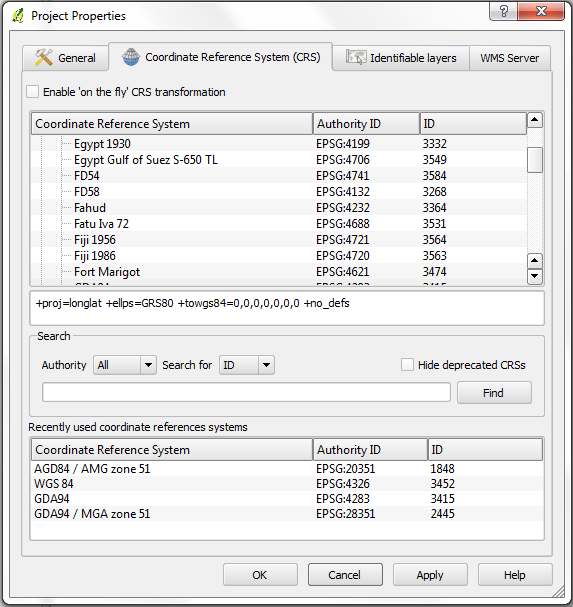
\includegraphics[clip=true, width=10cm]{projectionDialog}
   \caption{Finestra di dialogo per l'impostazione della proiezione \nixcaption}\label{fig:projections}
\end{figure}

\begin{enumerate}
\item \textbf{Abilita la riproiezione al volo}\index{Projections!enabling} -
questa casella di controllo è usata per attivare o disattivare la riproiezione OTF. 
Quando è deselezionata, ogni layer è tracciato usando le coordinate lette dal dato sorgente. 
Se abilitata, le coordinate di ogni layer sono riproiettate nel sistema di coordinate definito per la mappa.
\item \textbf{Coordinate di Riferimento spaziale} - è la lista di tutti i CRS supportati da QGIS, inclusi i
sistemi di coordinate geografiche, piane e quelli personalizzati. Per usare un CRS, selezionarlo
dalla lista espandendo il gruppo appropriato. Il CRS attivo è preselezionato.
\item \textbf{Stringa Proj4} - è la stringa CRS usata dal motore di proiezione Proj4. 
È un testo di sola lettura, a solo scopo informativo.
\item \textbf{Trova} - se si conosce il codice EPSG, l'identificatore o il nome del CRS che si vuole impostare, 
può essere usata questa area di ricerca per trovarlo nell'elenco, inserendo una voce di ricerca e facendo click 
su \button{Trova}. Usare la casella \checkbox{Nascondi i CRS sconsigliati} per mostrare solo le proiezioni attualmente approvate.
\item \textbf{Sistemi di riferimento usati di recente} - se ci sono dei CRS che vengono usati frequentemente 
nel lavoro quotidiano con i GIS, 
essi verranno visualizzati in questa tabella nella parte inferiore della finestra di dialogo. 
Basta fare click su una voce per impostare il CRS associato.
\end{enumerate}

\begin{Tip}
\caption{\textsc{Finestra di proprietà del Progetto}}
Se si apre la finestra \dialog{Proprietà progetto} dal menu \mainmenuopt{Modifica} (Gnome, OSX) 
o \mainmenuopt{Impostazioni} (KDE, Windows), bisogna fare click sulla scheda \tab{Sistema di 
coordinate di riferimento spaziale} (CRS) per visualizzare le impostazioni del CRS. Aprendo la 
finestra dall'icona \toolbtntwo{mIconProjectionEnabled}{Stato CRS}, verrà automaticamente aperta 
anche la scheda \tab{Sistema di coordinate di riferimento spaziale} (CRS).
\end{Tip}

\section{Sistemi di coordinate di riferimento personalizzati}\label{sec:customprojections}
\index{Projections!custom}

Se in QGIS non si trova il sistema di coordinate di riferimento di cui si necessita, 
è possibile definirne uno personalizzato. Per fare questo, selezionare 
\dropmenuopttwo{mIconNew}{CRS personalizzato} dal menu \mainmenuopt{Modifica} (Gnome, OSX) 
o \mainmenuopt{Impostazioni} (KDE, Windows). 
I CRS personalizzati sono salvati nel database utente di QGIS. Oltre ai CRS personalizzati, 
questo database contiene anche i segnalibri geospaziali e altri dati personalizzati dell'utente.

\begin{figure}[ht]
   \centering
   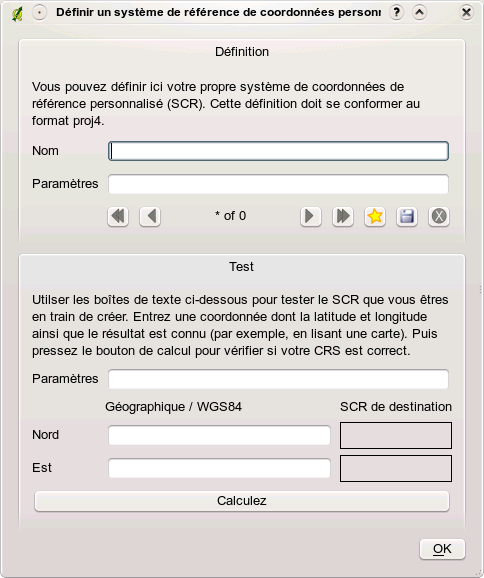
\includegraphics[clip=true, width=8cm]{customProjectionDialog}
   \caption{Finestra per i CRS personalizzati \nixcaption}\label{fig:customprojections}
\end{figure}

La definizione di un CRS personalizzato in QGIS richiede una buona comprensione delle librerie
Proj.4. Per iniziare, fare riferimento al documento "Cartographic Projection Procedures for the UNIX Environment - A User's Manual" di Gerald I. Evenden, U.S. Geological Survey Open-File Report 90-284, 1990 
(disponibile all'indirizzo \url{ftp://ftp.remotesensing.org/proj/OF90-284.pdf}). 
Questo manuale descrive l'uso di \usertext{proj.4} e delle relative utilità da riga di comando. 
I parametri cartografici usati da \usertext{proj.4} sono descritti nel manuale e sono identici a quelli usati da QGIS.

La finestra \dialog{Definizione Sistema Riferimento Spaziale Personalizzato} richiede solo due
parametri per definire un CRS personalizzato:
\begin{enumerate}
\item un nome descrittivo e
\item i parametri cartografici in formato PROJ.4.
\end{enumerate}
Per creare un nuovo CRS, fare click sul pulsante \toolbtntwo{mIconNew}{Nuovo} e inserire 
il nome descrittivo e i parametri CRS. Successivamente salvare il CRS facendo click sul pulsante \toolbtntwo{mActionFileSave}{Salva}.

Si noti che la voce \guilabel{Parametri} deve iniziare con un blocco \usertext{+proj=}, per rappresentare il nuovo CRS.

È possibile testare i parametri CRS per vedere se danno risultati validi facendo click sul pulsante
\button{Calcola} nella sezione \guiheading{Prova}, dopo aver incollato i parametri CRS personalizzati 
nel campo \guilabel{Parametri}.
Quindi, inserire dei valori noti di latitudine e longitudine nel sistema WGS 84 rispettivamente nei campi \guilabel{Nord} e \guilabel{Est}. 
Fare click su \button{Calcola} e confrontare i risultati con i valori noti nel sistema CRS personalizzato.

\FloatBarrier
